% Estas slides tienen que abrirse con el programa pdfpc que soporta videos embebidos. Para los videos se requiere ubuntu-restricted-extras. El comando es: pdfpc -g slides.pdf

% compress: Encabezado muestra solo la section actual
\documentclass[compress]{beamer}
\mode<presentation>

\usetheme{Copenhagen}
\useoutertheme{taihu}
\useinnertheme{rectangles}

% Itemize configuration
\setbeamertemplate{itemize item}[rectangle]
\setbeamertemplate{itemize subitem}[circle]
\setbeamertemplate{itemize subsubitem}[triangle]

\setbeamertemplate{navigation symbols}{} % Remover símbolos de navegación
\usefonttheme[onlymath]{serif} % Símbolos matemáticos en Serif

\setbeamertemplate{blocks}[rounded] % Block corners rounded
\setbeamercolor{block body}{bg=blue!12,fg=black} % Color of blocks

\usepackage{pdfpc-commands} % pdfpc movie commands
\usepackage[utf8]{inputenc}
\usepackage[spanish]{babel}
\usepackage[binary-units=true]{siunitx} % Para manejar las unidades
\usepackage{multirow}
\usepackage{multimedia}
\usepackage{graphicx}
\usepackage{xcolor}
\usepackage{booktabs} % \toprule

% Elimina la palabra 'Figura' del caption
\usepackage[caption=false]{subfig}
\setbeamertemplate{caption}{\raggedright\insertcaption\par}
\captionsetup[subfigure]{labelformat=empty} % Remover índice del caption de la subfigura

\usepackage{import} % Para el comando import (se usa para pdf_tex)

% Para notas personales en el pdfpc
\usepackage{pdfpcnotes}

%\AtBeginSection[]
%{
%   \begin{frame}
%       \frametitle{Índice}
%       \tableofcontents[currentsection]
%   \end{frame}
%}

\setbeamercovered{transparent}

\usepackage{amsmath}
\usepackage{amssymb}
\usepackage{amsopn}

% math
\renewcommand{\vec}[1]{\boldsymbol{\mathbf{#1}}}
\newcommand{\norm}[1]{\left\lVert#1\right\rVert}

% Declare arg max and arg min functionss
\DeclareMathOperator*{\argmax}{arg\,max}
\DeclareMathOperator*{\argmin}{arg\,min}

% Homogeneous decoration function
\newcommand{\homo}[1]{\dot{#1}}

% Declare projection as math function
\DeclareMathOperator{\proj}{proj}
\DeclareMathOperator{\disp}{disp}
\newcommand{\worldCoordSystem}{\mathrm{w}}
\newcommand{\cameraCoordSystem}{\mathrm{c}}
\newcommand{\point}{\vec{x}}
\newcommand{\worldPoint}{\point^{\mathrm{w}}}
\newcommand{\homoWorldPoint}{\homo{\point}^{\mathrm{w}}}
\newcommand{\cameraPoint}{\point^{\mathrm{c}}}
\newcommand{\hatCameraPoint}{\hat{\point}^{\mathrm{c}}}
\newcommand{\homoCameraPoint}{\homo{\point}^{\mathrm{c}}}
\newcommand{\measurement}{\vec{z}}
\newcommand{\prediction}{\hat{\vec{z}}}
\newcommand{\imagePoint}{\vec{u}}
\newcommand{\seMatrix}{\vec{E}}
\newcommand{\rotation}{\vec{R}}
\newcommand{\translation}{\vec{t}}
\newcommand{\intrinsicMatrix}{\vec{K}}
\newcommand{\principalPoint}{\vec{c}}
\newcommand{\reprojectionError}{u}
\newcommand{\projectionMatrix}{\vec{P}}
\newcommand{\cameraCenter}{\vec{o}}


% Dense Map
\newcommand{\current}{\mathrm{current}}
\newcommand{\previous}{\mathrm{previous}}
\newcommand{\fusion}{\mathrm{fusion}}
\newcommand{\inverseDepth}{\rho}
\newcommand{\plane}{\boldsymbol{\pi}}
\newcommand{\reference}{ref}


% scaled operators and letters to fancy view
\newcommand{\sminus}{\scalebox{0.5}[1.0]{$-$}}
\newcommand{\splus}{\scalebox{0.6}[0.6]{$+$}}
\newcommand{\curr}{c}
\newcommand{\sind}[1]{\scalebox{0.6}[0.6]{$#1$}}
\newcommand{\ind}[1]{\scalebox{0.7}[0.7]{$#1$}}

\newcommand{\keyframe}{\vec{K}}
\newcommand{\pointCloud}{\mathcal P}
\newcommand{\groundTruth}[1]{{#1}^{*}}

\newcommand{\update}[1]{\hat{#1}}

\newcommand{\position}{\vec{p}}
\newcommand{\map}{M}

\newcommand{\baseline}{b}
\newcommand{\focalDistance}{f}
\newcommand{\disparityMap}{\mathcal D}
\newcommand{\camera}{c}
\newcommand{\ray}{n}


\setbeamerfont{normal text}{size*={10}{10}}
\AtBeginDocument{\usebeamerfont{normal text}}

\title{Mapeo denso online sobre sistemas SLAM basados en visión estéreo}
\author{Ariel D'Alessandro}
\institute{Director: Taihú Pire. Co-Director: Rodrigo Baravalle. \\ \vspace{0.5cm} Tesina de Grado \\ Licenciatura en Ciencias de la Computación \\ FCEIA - UNR}
\titlegraphic{\includegraphics[width=0.14\textwidth]{images/logo-unr.png}}
\date{\scriptsize{22 de diciembre de 2017}}

\begin{document}

\frame{
	\titlepage
	\pnote{
		Soy Ariel y esta es mi tesina.\\
		Agradecer jurado y dcc: Ana, Pablo G., Pablo Pilotti, Juan Carlos Gómez, Claudia Deco, Directores.\\
	}
}


% Frame ---------------------------------------------------------------------
\begin{frame}
	\frametitle{Estructura de la presentación}
	\tableofcontents
	
	\pnote{
		Aportes 2,3,4.\\
	}
\end{frame}


\section{Introducción}


\subsection{Robótica móvil}


\begin{frame}
	\frametitle{Robots móviles}
	\pnote{
		Campo en desarrollo actualmente.\\
		Definición robot móvil.\\
		Numerosos ejemplos con distintas aplicaciones.\\
		Drones, automóviles, industriales\\
		curiosity (exploración), agricultura, acuáticos.\\
	}	
	
	\begin{figure}[!h]
		\centering
		\subfloat[] 
		{
			\includegraphics[width=0.33\columnwidth]{./images/introduction/drone.jpg}
		}
		\subfloat[] 
		{
			\includegraphics[width=0.33\columnwidth]{./images/introduction/GoogleCar.jpg}
		}
		\subfloat[] 
		{
			\includegraphics[width=0.16\columnwidth]{./images/introduction/industrial_robot.png}
		}\\
		\subfloat[] 
		{
			\includegraphics[width=0.33\columnwidth]{./images/introduction/curiosity.png}
		}
		\subfloat[] 
		{
			\includegraphics[width=0.33\columnwidth]{./images/introduction/hortibot.png}
		}
		\subfloat[]
		{
			\includegraphics[width=0.33\columnwidth]{./images/introduction/aqua2.png}
		}		 
	\end{figure}
\end{frame}


\begin{frame}
	\frametitle{Navegación autónoma}
	\pnote{
		Nos interesa que razonen sobre el entorno para navegar.\\
		No al micro management.\\
		Los dos primeros puntos son formulados en SLAM.\\
	}
	
	\begin{block}{}
		La navegación autónoma puede definirse a grandes rasgos como la capacidad de moverse de forma segura a lo largo de una trayectoria entre un punto de inicio y uno final [1].
	\end{block}
	\vspace{5mm}
	\begin{columns}
		\column{0.4\textwidth}
		\hspace{13pt}Pregunta:
		\begin{enumerate}
			\visible<2-7>{ \item[-] ¿Dónde estoy?}
			\visible<4-7>{\item[-] ¿Por dónde estoy yendo?}
			\visible<6-7>{\item[-] ¿Cómo llego hasta allí?}
		\end{enumerate}
		\column{0.6\textwidth}
		Respuesta:
		\begin{enumerate}[$\rightarrow$]
			\visible<3-7>{ \item  Cálculo de la posición (Localization)}
			\visible<5-7>{ \item  Representación del entorno (Mapping)}
			\visible<7-7>{\item  Planeamiento de movimiento (Motion planning)}
		\end{enumerate}
	\end{columns}
	\only<4>{}
	\vfill
	\begin{tiny}
		[1] J. J. Leonard - et al., ``Mobile robot localization by ...,'' IEEE Transactions on Robotics and Automation, 2002.
	\end{tiny}
\end{frame}


\subsection{SLAM}


% Frame ---------------------------------------------------------------------
\begin{frame}
	\frametitle{SLAM - Simultaneous Localisation and Mapping}
	\pnote{
		El robot determina su posición y orientación en base a estas.\\
		Construye incrementalmente un mapa del entorno, ubicando estas marcas en el mismo.\\
	}

	\begin{itemize}
        \item Sensores permiten detectar marcas naturales (\textbf{landmarks})
    \end{itemize}

	\vspace{-1em}
	\begin{figure}[!htb]
		\centering
		\subfloat[]{\includegraphics[width=0.6\columnwidth]{./introduction/slam-landmarks.pdf}}
		\hfill
	\end{figure}

\end{frame}


\begin{frame}
	\frametitle{Algunos de los sensores más utilizados}	
	\pnote{
		IR - GPS - IMU - encoders\\
		Sonar - Zed camera - Laser\\
	}
	
	\begin{figure}[!h]
		\centering
		\subfloat[] 
		{
			\includegraphics[width=0.15\columnwidth]{images/introduction/ir_sensor.png}
		}
		\subfloat[] 
		{
			\includegraphics[width=0.18\columnwidth]{images/introduction/gps.jpg}
		}
		\subfloat[] 
		{
			\includegraphics[width=0.18\columnwidth]{images/introduction/imu.jpg}
		}
		\subfloat[] 
		{
			\includegraphics[width=0.2\columnwidth]{images/introduction/encoders-04.jpg}
		}\\
		\subfloat[]
		{
			\includegraphics[width=0.22\columnwidth]{images/introduction/sonar.png}
		}
		\subfloat[]
		{
			\centering
			\includegraphics[width=0.3\columnwidth]{images/introduction/zed_camera2.png}
		}
		\subfloat[]
		{
			\includegraphics[width=0.16\columnwidth]{images/introduction/laser.jpg}
		}
	\end{figure}
\end{frame}


\subsection{SLAM Visual}


\begin{frame}
	\frametitle{SLAM Visual: Cámaras como sensores}
	
	¿Por qué utilizar cámaras?
       \begin{tabular}{cl}  
         \begin{tabular}{c}
           \includegraphics[width=0.3\columnwidth]{./images/robot-with-camera.jpg}
           \end{tabular}
           & \begin{tabular}{l}
             \parbox{0.5\linewidth}{
	            \begin{itemize}
	              	\pause
		            \item Rica información.
					\pause
		            \item Ambientes interiores y exteriores.
		            \pause
		            \item Sensores pasivos.
		            \pause
		            \item Bajo costo.
		            \pause
		            \item Portátiles.
		        \end{itemize}
		    }
        \end{tabular}  \\
	\end{tabular}
\end{frame}


\subsection{Cámaras}


\begin{frame}
	\frametitle{Reconstrucción 3D con una cámara}
	
	\pnote{
		Cámara = Mapeo punto 3D a píxel 2D\\
		Necesitamos 2 puntos de vista\\
		Necesitamos conocer el desplazamiento\\
	}
	% SPEECH:
	% hacer el ejemplo de cerrar un ojo y mover el dedo indice. Luego de mover el dedo caias veces notar que no conocemos su distancia.
	\only<1>{
		\begin{figure}[!h]
			\includegraphics[width=0.8\textwidth]{images/slam/monocularReconstruction1}
		\end{figure}
	}
	
	% SPEECH:
	% necesitamos dos puntos de vistas para poder realizar una reconstrucción 3D
	
	\only<2>{
		\begin{figure}[!h]
			\includegraphics[width=0.8\textwidth]{images/slam/monocularReconstruction2}
		\end{figure}
	}
	
	
	% SPEECH:
	% pero si estamos usando una sola camara y la movemos para tener dos puntos de vistas distintos, tenemos que saber cuanto se desplazo. Caso contrio, no vamos a poder saber si nos movimos poco, o si nos movimos mucho y las cosas estan muy lejos.
	
	\only<3>{
		\begin{figure}[!h]
			\includegraphics[width=0.8\textwidth]{images/slam/monocularReconstruction3}
		\end{figure}
	}
	
	\begin{block}{}
		Al utilizar una cámara, hay una ambig\"{u}edad sobre la escena que se esta observando.
	\end{block}
	
\end{frame}


\begin{frame}
	\frametitle{¿Y si tenemos dos cámaras?}
	
	\pnote{
		Permiten recuperar la profundidad de la escena con una única captura.\\
		Permiten conocer la escala real de la escena observada.\\
	}
	
	\begin{figure}[!h]
		\includegraphics[width=0.6\textwidth]{images/slam/stereoReconstruction}
	\end{figure}
	
	\begin{block}{}
		Si tenemos {\bf dos cámaras}, y se conoce la posición de una con respecto a la otra, es posible realizar una reconstrucción 3D sin ambig\"{u}edades.
	\end{block}
	
\end{frame}


% Frame ---------------------------------------------------------------------
\begin{frame}
    \frametitle{Geometría estéreo: Disparidad}
    \pnote{
	    Distancia existente entre las proyecciones de las diferentes cámaras.\\
	    La profundidad z es inversamente proporcional a la disparidad d.\\
    }
    
    \begin{figure}[!htb]
        \centering
        \subfloat[]{
        \hspace{-3.0em}
        \includegraphics[width=1.15\columnwidth]{./images/disparity_sketch.jpeg}}
        \hfill
        \centering

        \hfill
    \end{figure}

\end{frame}


% Frame ---------------------------------------------------------------------
\begin{frame}
    \frametitle{Cierre y Motivación}
    \pnote{
    	Importancia de Robótica móvily Navegación autónoma.\\
		SLAM y SLAM Visual.\\
		Trayectoria seguro: mapa denso!\\
		Pasamos al aporte y al método\\
		No GPU!!!\\
    }
    
    \begin{block}{}
    \centering
	Mapeo denso online sobre sistemas SLAM basados en visión estéreo
	\end{block}

	\begin{figure}[!htb]
		\captionsetup{justification=centering}
		\subfloat[S-PTAM]{\includegraphics[width=0.4\columnwidth,height=2.5cm]{./introduction/sptam-map.png}
		}
		\hfil
		\subfloat[S-PTAM Denso]{\includegraphics[width=0.4\columnwidth,height=2.5cm]{./introduction/dense-map.png}
		}
	\end{figure}
	
\end{frame}


\section{S-PTAM Denso}


\subsection{S-PTAM}


\fullFrameMovie[loop]{~/Videos/S-PTAM.mkv}{./images/S-PTAM-video-cover.png}{
	\frametitle{S-PTAM: Stereo Parallel Tracking and Mapping}
	\pnote{
    	Sensor: Cámara estéreo\\
		Construye y mantiene un mapa disperso del entorno.\\
        Sistema SLAM basado en features.\\
		Basado en keyframes.\\
        Fuertemente paralelizado: tracking, local mapping y loop closing.\\
        Real-time incluso en trayectorias largas.\\
        Código open-source en ROS (GPLv3) https://github.com/lrse/sptam\\
	}

}


\subsection{Funcionamiento}


% Frame ---------------------------------------------------------------------
\begin{frame}
	\frametitle{S-PTAM Denso}
	\pnote{
		Aporte de la tesina.\\
		Breve resumen.\\
	}	
	
	\begin{figure}[htb]
		\centering
		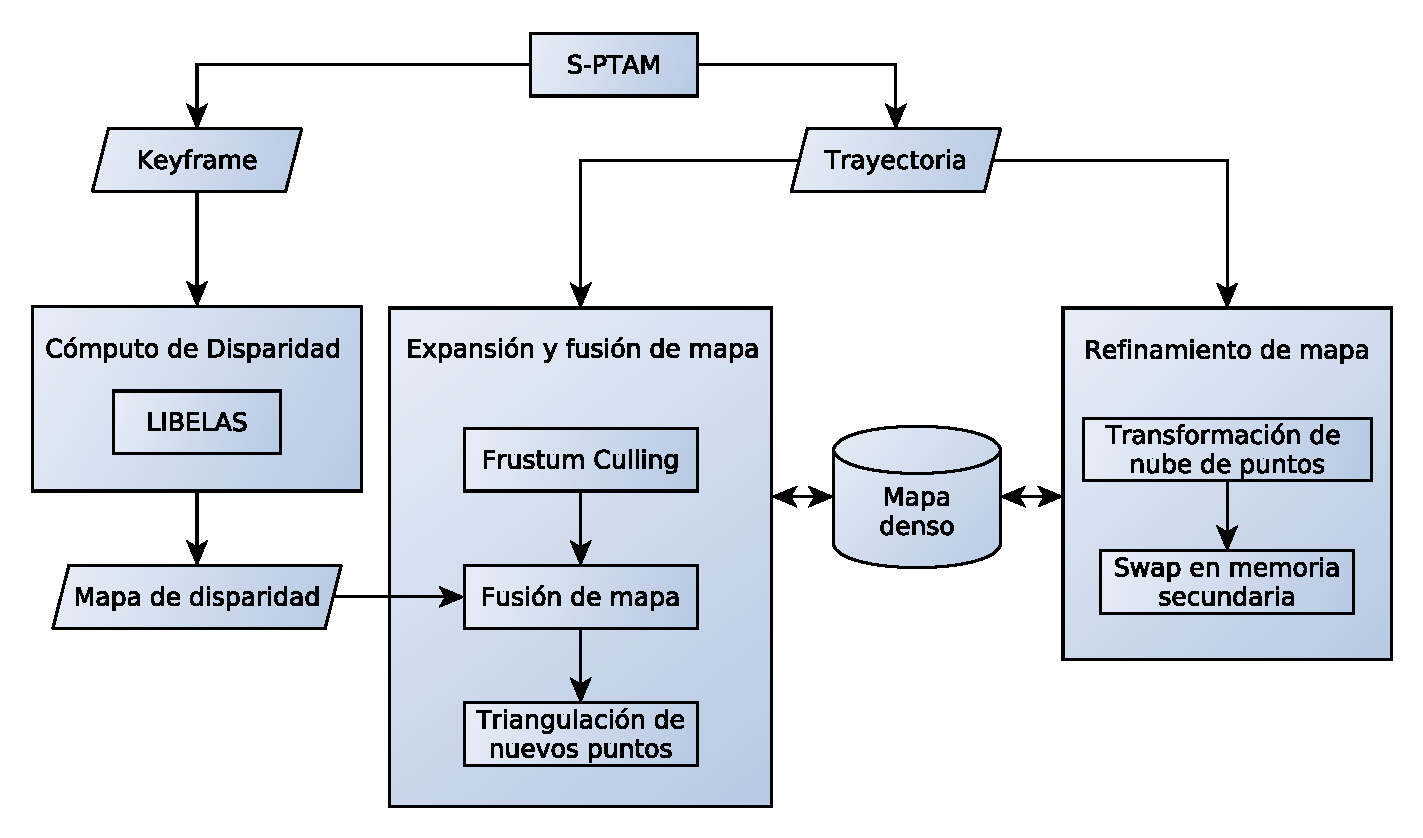
\includegraphics[width=1.0\columnwidth]{./method/metodo-diagram.pdf}
		\hfill
	\end{figure}
\end{frame}


% Frame ---------------------------------------------------------------------
\begin{frame}
	\frametitle{Mapa de disparidad}
	\pnote{
		LIBELAS: librería mapa denso.\\
		Usa todos los píxeles, contiene error (cielo).\\
	}	

	\begin{itemize}
		\item Computa mapa de disparidad del \emph{keyframe} actual $\keyframe_{j}$.
	\end{itemize}
	
	\begin{figure}[htb]
		\centering
		\includegraphics[width=0.4\columnwidth]{method/libelas_merge_kitti04_22.jpg}
		\caption{Mapa de disparidad LIBELAS - Dataset KITTI}
	\end{figure}

	\vspace{-1em}

	\begin{figure}[htb]
		\centering
		\includegraphics[width=0.4\columnwidth]{method/libelas_merge_tsukuba_222.jpg}
		\caption{Mapa de disparidad LIBELAS - Dataset Tsukuba}
	\end{figure}

	\begin{itemize}
		\item Colores: (rojo: mayor disparidad, azul: menor disparidad).
	\end{itemize}
	
\end{frame}


% Frame ---------------------------------------------------------------------
\begin{frame}
	\frametitle{Expansión y fusión de mapa: Heurística de fusión}
	\begin{figure}[htb]
		\centering
		\includegraphics[width=\columnwidth]{./method/metodo-fusion-spa.pdf}
	\end{figure}
	\begin{block}{Caso 1}
		Los puntos coinciden por su distancia eclideana y se \textbf{fusionan} en $\point_{fusion}$.
	\end{block}
\end{frame}


% Frame ---------------------------------------------------------------------
\begin{frame}
	\frametitle{Expansión y fusión de mapa: Heurística de fusión}
	\begin{figure}[htb]
		\centering
		\includegraphics[width=\columnwidth]{./method/metodo-fusion-spa-caso-1.pdf}
	\end{figure}
	\begin{block}{Caso 2}
		Los puntos \textbf{no} son coincidentes y el nuevo punto ($\point_{actual}$) \textbf{ocluye} al punto ($\point_{previo}$) del mapa.
	\end{block}
\end{frame}


% Frame ---------------------------------------------------------------------
\begin{frame}
	\frametitle{Expansión y fusión de mapa: Heurística de fusión}
	\begin{figure}[htb]
		\centering
		\includegraphics[width=\columnwidth]{./method/metodo-fusion-spa-caso-2.pdf}
	\end{figure}
	\begin{block}{Caso 3}
		Los puntos \textbf{no} son coincidentes y el nuevo punto ($\point_{actual}$) está \textbf{detrás} del punto ($\point_{previo}$) del mapa.  \textbf{Posible outlier!}
	\end{block}
\end{frame}


\begin{frame}
	\frametitle{Refinamiento de mapa}
	
	\pnote{
		Transforma nubes de puntos cuando la posición del keyframe asociado es actualizada.\\
		Comportamiento esperable en sistemas de SLAM, que refinan la trayectoria a lo largo de la secuencia.\\
		Nubes de puntos en RAM hasta que salen del mapa local.\\
		Permite correr en secuencias de extensa longitud.\\
	}    
	
       \begin{tabular}{cl}  
           \begin{tabular}{c}
           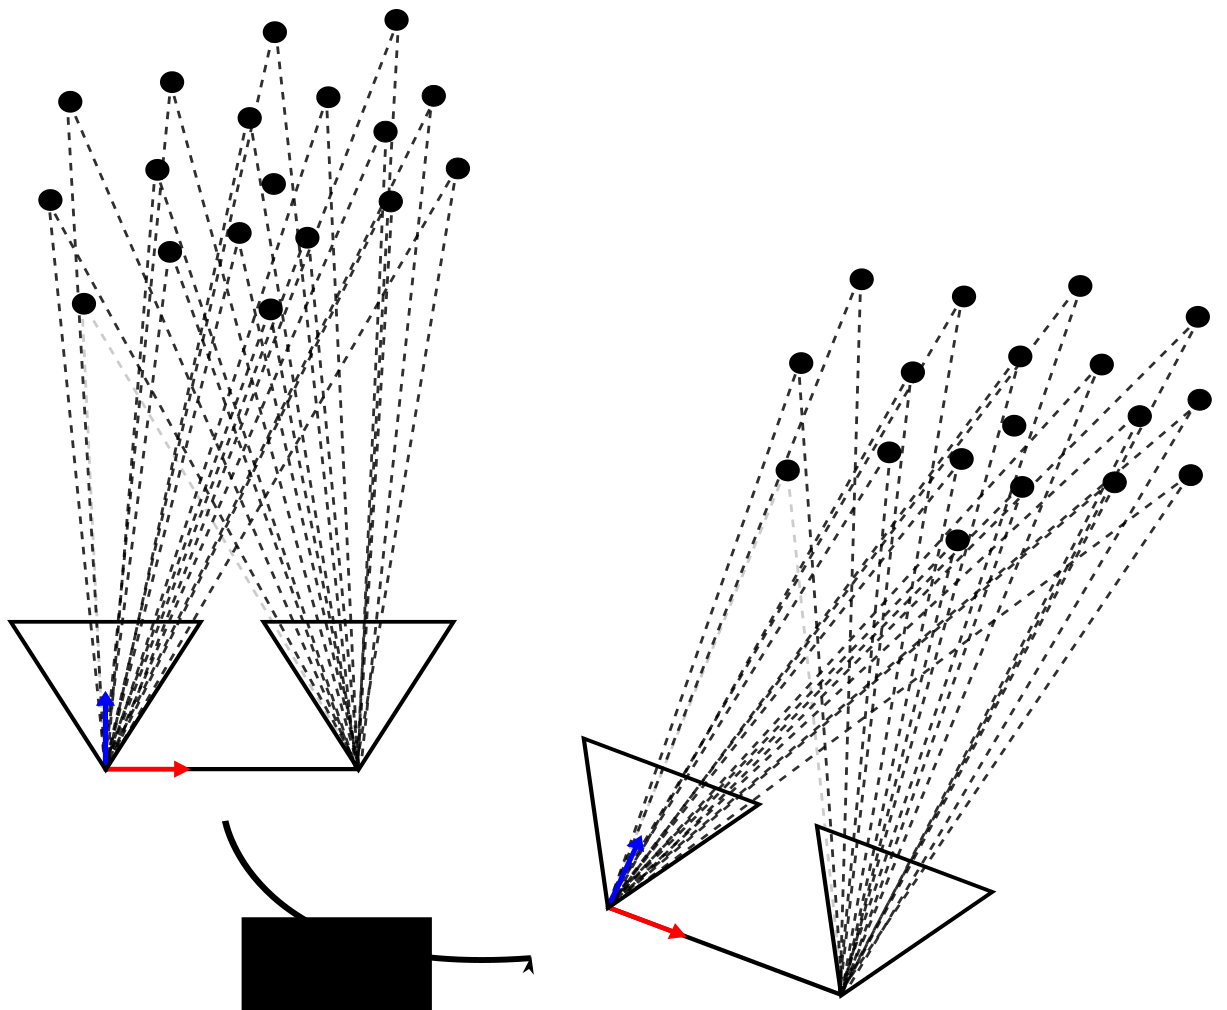
\includegraphics[width=0.5\columnwidth]{./images/point_cloud_refinement.pdf}
           \end{tabular}
           & \begin{tabular}{l}
             \parbox{0.5\linewidth}{
	            \begin{itemize}
	            	\item Refinamiento de nubes de puntos.
	            	\item Swapping del mapa en memoria secundaria.
		        \end{itemize}
		    }
			\end{tabular}
		\end{tabular}
		
		\begin{figure}[!htb]
		\captionsetup{justification=centering}
		\subfloat[SWAP memory]{
			\includegraphics[width=0.15\columnwidth]{./images/swap-memory.png}
		}
		\end{figure}
\end{frame}


\subsection{Implementación}


% Frame ---------------------------------------------------------------------
\begin{frame}
	\frametitle{Framework}
	

	\begin{figure}[htb]
		\subfloat[] {
			\begin{tabular}[b]{c}
				\centering
				$\vcenter{\hbox{\includegraphics[width=0.15\columnwidth]{./method/opencv.png}}}$
				\hspace{1em}
				$\vcenter{\hbox{\includegraphics[width=0.40\columnwidth]{./method/ros.png}}}$
				\hspace{1em}
				$\vcenter{\hbox{\includegraphics[width=0.28\columnwidth]{./method/pcl.png}}}$
			\end{tabular}
		}
	\end{figure}
	
	\vfill
	\begin{tiny}
		Código fuente disponible públicamente bajo licencia (GPLv3) \url{https://github.com/CIFASIS/dense-sptam}.
	\end{tiny}
	
	\pnote{
		Conjunto de frameworks para desarrollo de software en robótica.\\
		Abstracción del hardware.\\
	    Control de dispositivos de bajo nivel.\\
	    Arquitectura: Cada nodo es una unidad de ejecución. Comunicación entre nodos mediante mensajes.
		Mantenimiento de paquetes.\\
	    Utilizado en la comunidad robótica.\\
		Implementado como un nodo ROS.\\
		OpenCV: manejo y codificación de imágenes.\\
		Point Cloud Library (PCL): manejo de nubes de puntos.\\
		LIBELAS: cómputo de mapas de disparidad.\\
		Compuesto de 3 hilos de ejecución paralela.\\
	}

\end{frame}


\section{Evaluación}


\subsection{Datasets}


% Frame ---------------------------------------------------------------------
\begin{frame}
	\frametitle{Dataset KITTI}

	\begin{figure}
		\subfloat[] {
			\includegraphics[width=0.3\columnwidth]{./images/kitti_sensors}
		}\hfill{}
		\subfloat[] {
			\begin{tabular}[b]{c}%
				\includegraphics[width=0.3\columnwidth]{./images/kitti01}\thickspace\includegraphics[width=0.3\columnwidth]{./images/kitti02}\\
				\includegraphics[width=0.3\columnwidth]{./images/kitti03}\thickspace\includegraphics[width=0.3\columnwidth]{./images/kitti04}\\
				\includegraphics[width=0.3\columnwidth]{./images/kitti05}\thickspace\includegraphics[width=0.3\columnwidth]{./images/kitti06}
			\end{tabular}
		}
	\end{figure}

	\begin{itemize}
        \item Ambientes exteriores (trayectorias de varios kilómetros)
        \item 1344$\times$391@10Hz, baseline: 60cm
    \end{itemize}

\end{frame}


% Frame ---------------------------------------------------------------------
\begin{frame}
	\frametitle{Dataset Tsukuba}

	\begin{figure}
		\subfloat[] {
			\includegraphics[width=0.41\columnwidth]{./images/tsukuba_dataset}
		}\hspace{0.2cm}
		\subfloat[] {
			\begin{tabular}[b]{c}%
				\includegraphics[width=0.2\columnwidth]{./images/tsukuba_sample1}\thickspace\includegraphics[width=0.2\columnwidth]{./images/tsukuba_sample2}\\
				\includegraphics[width=0.2\columnwidth]{./images/tsukuba_sample3}\thickspace\includegraphics[width=0.2\columnwidth]{./images/tsukuba_sample4}
			\end{tabular}
		}
	\end{figure}
	
	\begin{itemize}
        \item Ambiente interior (sintético)
        \item 640$\times$480@30Hz, baseline: 10cm
    \end{itemize}
    
\end{frame}


% Frame ---------------------------------------------------------------------
\begin{frame}
	\frametitle{Reconstrucción 3D: Tsukuba}
	\begin{figure}
		\subfloat[] {
			\begin{tabular}[b]{c}
				\includegraphics[width=0.3\columnwidth,height=3.0cm]{./images/tsukuba_3d_1}\thickspace
				\includegraphics[width=0.3\columnwidth,height=3.0cm]{./images/tsukuba_3d_2}\thickspace
				\includegraphics[width=0.3\columnwidth,height=3.0cm]{./images/tsukuba_3d_3}
			\end{tabular}
		}
	\end{figure}
\end{frame}

\fullFrameMovie[loop]{~/Videos/Dense-online.mp4}{./images/Dense-online.png}{
	\frametitle{Reconstrucción 3D: KITTI}
	\pnote{
		Primero online.
		Downsampleo.
		Re-publica la nube local todo el tiempo. Más lento.		
		Después offline.
	}

}

\subsection{Resultados}


% Frame ---------------------------------------------------------------------
\begin{frame}
	\frametitle{KITTI: error de reconstrucción}
	\pnote{
		Comparación de mapas de profundidad.\\
		Proyectamos nubes de puntos.\\
		LIBELAS.\\
		GT en KITTI y Tsukuba.\\
	}	
	
	\vspace{-2em}
	\begin{figure}
		\subfloat[Imagen izquierda]{
			\begin{tabular}[b]{c}
				\includegraphics[width=0.45\columnwidth]{./experiments/kitti06_frame612_rgb.png}
			\end{tabular}
		}\thickspace
		\subfloat[Ground-Truth]{
			\begin{tabular}[b]{c}
				\includegraphics[width=0.45\columnwidth]{./experiments/kitti06_frame612_gt_high50.png}
			\end{tabular}
		}
	\end{figure}
	\vspace{-2em}
	\begin{figure}
		\subfloat[Mapa profundidad LIBELAS]{
			\begin{tabular}[b]{c}
				\includegraphics[width=0.45\columnwidth]{./experiments/kitti06_frame612_libelas_depth_high50-m.png}
			\end{tabular}
		}\thickspace
		\subfloat[Error mapa profundidad LIBELAS]{
			\begin{tabular}[b]{c}
				\includegraphics[width=0.45\columnwidth]{./experiments/kitti06_frame612_libelas_error_high50-m.png}
			\end{tabular}
		}
	\end{figure}
	\vspace{-2em}
	\begin{figure}
		\subfloat[Mapa profundidad S-PTAM Denso]{
			\begin{tabular}[b]{c}
				\includegraphics[width=0.45\columnwidth]{./experiments/kitti06_frame612_dense_high50-m.png}
			\end{tabular}
		}\thickspace
		\subfloat[Error mapa profundidad S-PTAM Denso]{
			\begin{tabular}[b]{c}
				\includegraphics[width=0.45\columnwidth]{./experiments/kitti06_frame612_error_high50-m.png}
			\end{tabular}
		}
	\end{figure}
	\vspace{-2em}
	\begin{figure}
		\subfloat[]{
			\begin{tabular}[b]{c}
				\includegraphics[width=0.60\columnwidth]{./experiments/high50_bar.pdf}
			\end{tabular}
		}
	\end{figure}
\end{frame}


% Frame ---------------------------------------------------------------------
\begin{frame}
	\frametitle{Tsukuba: error de reconstrucción}
	\vspace{-1em}
	\begin{figure}
		\captionsetup{justification=centering}
		\subfloat[Imagen izquierda]{
			\begin{tabular}[b]{c}
				\includegraphics[width=0.25\columnwidth]{./experiments/tsukuba_frame807_rgb.png}
			\end{tabular}
		}\thickspace
		\subfloat[Mapa profundidad LIBELAS]{
			\begin{tabular}[b]{c}
				\includegraphics[width=0.25\columnwidth]{./experiments/tsukuba_frame807_libelas_depth_high6.png}
			\end{tabular}
		}\thickspace
		\subfloat[Mapa profundidad S-PTAM Denso]{
			\begin{tabular}[b]{c}
				\includegraphics[width=0.25\columnwidth]{./experiments/tsukuba_frame807_dense_high6.png}
			\end{tabular}
		}
	\end{figure}
	\vspace{-2em}
	\begin{figure}
		\captionsetup{justification=centering}
		\subfloat[Ground-Truth]{
			\begin{tabular}[b]{c}
				\includegraphics[width=0.25\columnwidth]{experiments/tsukuba_frame807_gt_high6.png}
			\end{tabular}
		}\thickspace
		\subfloat[Error mapa profundidad LIBELAS]{
			\begin{tabular}[b]{c}
				\includegraphics[width=0.25\columnwidth]{./experiments/tsukuba_frame807_libelas_error_high6-m.png}
			\end{tabular}
		}\thickspace
		\subfloat[Error mapa profundidad S-PTAM Denso]{
			\begin{tabular}[b]{c}
				\includegraphics[width=0.25\columnwidth]{./experiments/tsukuba_frame807_error_high6-m.png}
			\end{tabular}
		}
	\end{figure}
	\vspace{-2em}
	\begin{figure}
		\subfloat[]{
			\begin{tabular}[b]{c}
				\includegraphics[width=0.60\columnwidth]{./experiments/high6_bar.pdf}
			\end{tabular}
		}
	\end{figure}
\end{frame}


% Frame ---------------------------------------------------------------------
\begin{frame}
	\frametitle{KITTI 06: error de mediana}
	\centering
	Error (profundidad vs. error) en la secuencia 06 del Dataset KITTI.
	\begin{figure}[!htb]
		\captionsetup{justification=centering}
		\subfloat[Error en LIBELAS]{\includegraphics[width=0.48\columnwidth]{./experiments/kitti06_libelas_boxplot.png}%
		}
		\hfil
		\subfloat[Error en S-PTAM Denso]{\includegraphics[width=0.48\columnwidth]{./experiments/kitti06_dense_boxplot.png}%
		}
	\end{figure}
\end{frame}


% Frame ---------------------------------------------------------------------
\begin{frame}
	\frametitle{KITTI 06: error de mediana}
	\vspace{-2em}
	\begin{figure}[!htb]
		\captionsetup{justification=centering}
		\subfloat[Comparación de mediana de error entre LIBELAS y S-PTAM Denso (profundidad vs. error) en la secuencia 06 del Dataset KITTI.] {
			\includegraphics[width=0.8\columnwidth]{./experiments/medians_comparison_kitti.png}%
		}
	\end{figure}
\end{frame}


% Frame ---------------------------------------------------------------------
\begin{frame}
	\frametitle{Tsukuba: error de mediana}
	\centering
	Error (profundidad vs. error) en el Dataset Tsukuba.
	\begin{figure}[!htb]
		\captionsetup{justification=centering}
		\subfloat[Error en LIBELAS]{\includegraphics[width=0.48\columnwidth]{./experiments/tsukuba_libelas_boxplot.png}%
		}
		\hfil
		\subfloat[Error en S-PTAM Denso]{\includegraphics[width=0.48\columnwidth]{./experiments/tsukuba_dense_boxplot.png}%
		}
	\end{figure}
\end{frame}


% Frame ---------------------------------------------------------------------
\begin{frame}
	\frametitle{Tsukuba: error de mediana}
	\vspace{-2em}
	\begin{figure}[!htb]
		\captionsetup{justification=centering}
		\subfloat[Comparación de mediana de error entre LIBELAS y S-PTAM Denso (profundidad vs. error) en el Dataset Tsukuba.] {
			\includegraphics[width=0.8\columnwidth]{./experiments/medians_comparison_tsukuba.png}%
		}
	\end{figure}
\end{frame}


% Frame ---------------------------------------------------------------------
\begin{frame}
	\frametitle{Cantidad de puntos}
	\begin{figure}[!htb]
		\centering
		\subfloat[KITTI]{\includegraphics[width=0.5\columnwidth]{./experiments/points_kitti06}%
			}
		\hfil
		\subfloat[Tsukuba]{\includegraphics[width=0.5\columnwidth]{./experiments/points_tsukuba}%
			}
	\end{figure}
\end{frame}


% Frame ---------------------------------------------------------------------
\fullFrameMovie[loop]{~/Videos/Dense-offline.mp4}{./images/Dense-offline.png}{
	\frametitle{S-PTAM Denso!}
}


\section{Conclusiones y trabajos futuros}


% Frame ---------------------------------------------------------------------
\begin{frame}
	\frametitle{Conclusiones}
	\begin{itemize}
		\item Sistema de SLAM capaz de generar un \textbf{mapa local denso} de manera \textbf{online}.
        \item La \textbf{precisión} es útil para tareas de navegación.
        \item Funciona incluso en trayectorias de \textbf{grandes dimensiones}.
        \item Evaluado en \textbf{datasets} públicos: KITTI (outdoors) y Tsukuba (indoors).
	    \item Código open-source en ROS (GPLv3) \url{https://github.com/CIFASIS/dense-sptam}
	    \item Nodo ROS \textbf{reutilizable}, desacoplado del sistema de SLAM disperso.
	  	\item Explota \textbf{paralelismo}.
	  	\item No requiere \textbf{GPU}.
	\end{itemize}
\end{frame}


% Frame ---------------------------------------------------------------------
\begin{frame}
	\frametitle{Trabajo Futuro}
	\begin{itemize}
		\item Incluir información de \textbf{apariencia} en la heurística.
		\item Ampliar \textbf{criterio} de correspondencias a considerar un entorno alrededor del píxel proyectado.
		\item Simplificar las nubes de puntos mediante la detección de regiones \textbf{planares}.
		\item Características visuales de alto nivel: información semántica, machine-learning.
		\item Utilizar \textbf{covisibilidad} en el mapa local.
	\end{itemize}
\end{frame}


\section*{}


\setbeamercovered{invisible}


% Frame ---------------------------------------------------------------------
\begin{frame}
    \frametitle{Publicaciones}

	\begin{itemize}
		\item A. D'Alessandro, T. Pire, R. Baravalle: \textbf{Hacia una densificación de sistemas SLAM dispersos basados en visión estéreo}. En IX Jornadas Argentinas de Robótica (JAR) 2017. 15, 16 y 17 de Noviembre de 2017. Facultad Regional Córdoba, Córdoba, Universidad Tecnológica Nacional. Noviembre 2017.
	\end{itemize}
    
\end{frame}


\begin{frame}
	\centering
	\Large{Muchísimas gracias!}	
	\\
	\pause{Preguntas?}	
	\vspace{2cm}
\end{frame}


% Frame ---------------------------------------------------------------------
\begin{frame}
\frametitle{Modelo de cámara}

\begin{block}{Definición - Cámara}
Una cámara es definida matemáticamente como una correspondencia entre el mundo 3D y una imagen 2D. Es decir, un mapeo entre puntos del mundo 3D $\point$ y puntos de la imagen $\imagePoint$:
\begin{equation}
\point=\begin{bmatrix}x\\
y\\
z
\end{bmatrix}\longmapsto
\imagePoint=\begin{bmatrix}u\\
v
\end{bmatrix}
\end{equation}
\end{block}

\end{frame}


% Frame ---------------------------------------------------------------------
\begin{frame}
\frametitle{Modelo de cámara pinhole}

\begin{block}{Cámara pinhole}
El punto de la imagen $\imagePoint=\begin{bmatrix}u & v\end{bmatrix}^{\top}$ es determinado como la intersección entre el \emph{plano de la imagen} y el rayo que une el punto del mundo 3D $\point=\begin{bmatrix}x & y & z\end{bmatrix}^{\top}$ con el \emph{centro focal} $\cameraCenter$ de la cámara.
\end{block}

\begin{figure}[!htb]
	\centering
	\subfloat[]{\includegraphics[width=0.5\columnwidth]{./cameras/pinhole_camera_model.pdf}}%
	\hfill
\end{figure}

\end{frame}


% Frame ---------------------------------------------------------------------
\begin{frame}
\frametitle{Modelo de cámara pinhole}

\begin{block}{Proyección central}
Asumiendo el centro focal en el origen de coordenadas y el plano de la imagen $Z=f$:

\begin{equation}
\begin{bmatrix}x\\
y\\
z
\end{bmatrix}\longmapsto\begin{bmatrix}fx/z\\
fy/z
\end{bmatrix}
\end{equation}

\end{block}

\begin{figure}[!htb]
	\centering
	\subfloat[]{\includegraphics[width=0.5\columnwidth]{./cameras/pinhole_camera_model.pdf}}%
	\hfill
	\centering
	\subfloat[]{\includegraphics[width=0.5\columnwidth]{./cameras/pinhole_camera_model2.pdf}}%
	\hfill
\end{figure}

\end{frame}


% Frame ---------------------------------------------------------------------
\begin{frame}
\frametitle{Triangulación estéreo}

Proyecciones correspondientes $\imagePoint_{l}=\begin{bmatrix}u_{l} & v_{l}\end{bmatrix}$ y $\imagePoint_{r}=\begin{bmatrix}u_{r} & v_{r}\end{bmatrix}$ sobre los planos focales de la imagen izquierda y derecha respectivamente,
la posición del punto $\point$ puede ser derivada.

\begin{equation}
\frac{b}{z}=\frac{(b+u_{r})-u_{l}}{z-f}
\end{equation}

\begin{figure}[!htb]
	\centering
	\subfloat[]{\includegraphics[width=0.5\columnwidth]{./cameras/stereo_triangulation.pdf}}%
	\hfill
	\centering
	\subfloat[]{\includegraphics[width=0.5\columnwidth]{./cameras/stereo_triangulation2.pdf}}%
	\hfill
\end{figure}
\end{frame}


% Frame ---------------------------------------------------------------------
\begin{frame}
\frametitle{Triangulación estéreo}

\begin{equation}
\frac{x}{z}=\frac{u_{l}-c_{u}}{f}\qquad\frac{y}{z}=\frac{v_{l}-c_{v}}{f}
\end{equation}

\begin{equation}
\begin{aligned}x=\frac{(u_{l}-c_{u})z}{f}\;\qquad
y=\frac{(v_{l}-c_{v})z}{f}\;\qquad
z=\frac{bf}{u_{l}-u_{r}}\;
\end{aligned}
\end{equation}

\begin{figure}[!htb]
	\centering
	\subfloat[]{\includegraphics[width=0.5\columnwidth]{./cameras/stereo_triangulation.pdf}}%
	\hfill
	\centering
	\subfloat[]{\includegraphics[width=0.5\columnwidth]{./cameras/stereo_triangulation2.pdf}}%
	\hfill
\end{figure}
\end{frame}


% Frame ---------------------------------------------------------------------
\begin{frame}
\frametitle{Disparidad}

\begin{block}{Definición - Disparidad}
La disparidad $d$ es definida como la distancia existente entre las proyecciones de las diferentes cámaras.
\begin{equation}
d=u_{l}-u_{r}=\frac{bf}{z}
\end{equation}
\end{block}

\textbf{Nota}: la profundidad $z$ es inversamente proporcional a la disparidad $d$.

\end{frame}

%%% READY

\begin{frame}
\frametitle{Modelo de cámara pinhole}

\pnote{* Lo anterior asume que el origen de coordenadas del plano de la imagen se encuentra en el punto principal. En la práctica, esto no siempre se cumple.}

\pnote{* Explicar representación en coordenadas homogéneas.}

Siendo $\begin{bmatrix}c_{u} & c_{v}\end{bmatrix}^{\top}$ la posición del punto principal.
\begin{equation}
\begin{bmatrix}x\\
y\\
z
\end{bmatrix}\longmapsto\begin{bmatrix}fx/z+c_{u}\\
fy/z+c_{v}
\end{bmatrix}
\end{equation}

En coordenadas homogéneas:

\begin{equation}
\begin{bmatrix}x\\
y\\
z\\
1
\end{bmatrix}\longmapsto\begin{bmatrix}fx+zc_{u}\\
fy+zc_{v}\\
z
\end{bmatrix}=\begin{bmatrix}f &  & c_{u} & 0\\
 & f & c_{v} & 0\\
 &  & 1 & 0
\end{bmatrix}\begin{bmatrix}x\\
y\\
z\\
1
\end{bmatrix}
\end{equation}

\begin{block}{Matriz de calibración intrínseca $\intrinsicMatrix$}
\begin{equation}
\intrinsicMatrix=\begin{bmatrix}f & 0 & c_{u}\\
0 & f & c_{v}\\
0 & 0 & 1
\end{bmatrix}
\end{equation}
\begin{equation}
\homo{\imagePoint}=\intrinsicMatrix\begin{bmatrix}\vec{{I}} & \vec{{0}}\end{bmatrix}\homo{\point}
\end{equation}
\end{block}

\end{frame}


\begin{frame}
\frametitle{Modelo de cámara pinhole}

\pnote{* Las ecuaciones anteriores deben extenderse agregando la transformación existente entre los sistemas de coordenadas de la cámara y el mundo.}

\pnote{* R es una matriz de rotación y t un vector de traslación.}

Puntos expresados en referencia al sistema de coordenadas del \textit{mundo}. La cámara no se encuentra necesariamente ubicada en el centro de este.

\begin{figure}[!htb]
	\centering
	\subfloat[]{\includegraphics[width=0.4\columnwidth]{./cameras/camera_coord_system.pdf}}%
	\hfill
\end{figure}

\begin{block}{}
\begin{equation}
\homoCameraPoint=\begin{bmatrix}\rotation & \translation\\
0 & 1
\end{bmatrix}\begin{bmatrix}x\\
y\\
z\\
1
\end{bmatrix}=\seMatrix^{\mathrm{c}\mathrm{w}}\homoWorldPoint\;.
\end{equation}
\end{block}

\end{frame}


\begin{frame}
\frametitle{Modelo de cámara pinhole}

De esta manera, es posible proyectar cualquier punto 3D
$\homoWorldPoint$ en el sistema de coordenadas del mundo al correspondiente
punto $\homo{\imagePoint}$ en el plano de la imagen mediante:

\begin{block}{Matriz de proyección \textmd{$\projectionMatrix$}}
\begin{equation}
\projectionMatrix=\intrinsicMatrix\begin{bmatrix}\rotation & \translation\end{bmatrix}
\end{equation}
\begin{equation}
\homo{\imagePoint}=\projectionMatrix\homoWorldPoint
\end{equation}
\end{block}

\end{frame}


\begin{frame}
\frametitle{Modelo de cámara estéreo}

\begin{block}{Geometría epipolar}

\pnote{* La geometría proyectiva intrínseca entre dos cámaras es conocida como geometría epipolar.}

\pnote{* Esta es independiente de la escena observada y depende únicamente de los parámetros internos geometría epipolar y las posiciones relativas de las cámaras involucradas.}

Cualquier punto 3D $\point$ en el espacio, sus proyecciones $\imagePoint$ y $\imagePoint^{\prime}$ en los planos de las imágenes y los centros focales de las cámaras, pertenecen a un mismo plano $\vec{\pi}$.
De manera análoga, los rayos re-proyectados desde $\imagePoint$ y $\imagePoint^{\prime}$ se intersectan en $\point$, son coplanares y yacen sobre $\vec{\pi}$.
\end{block}

\begin{figure}[!htb]
	\centering
	\subfloat[]{\includegraphics[width=0.5\columnwidth]{./cameras/pencil_of_planes.pdf}}%
	\hfill
	\centering
	\subfloat[]{\includegraphics[width=0.5\columnwidth]{./cameras/epipolar_plane.pdf}}%
	\hfill
\end{figure}
\end{frame}


\begin{frame}
\frametitle{Modelo de cámara estéreo}

\pnote{* La búsqueda del correspondiente al punto u no necesita cubrir el plano de la imagen completo sino que puede restringirse a la línea epipolar l.}

\pnote{* La línea epipolar es generada por la proyección del rayo, re-proyectado desde u, sobre el plano focal de la segunda imagen.}

Búsqueda de correspondencias sobre la línea epipolar.

\begin{figure}[!htb]
	\centering
	\subfloat[]{\includegraphics[width=0.5\columnwidth]{./cameras/epipolar_line.pdf}}%
	\hfill
\end{figure}
\end{frame}


\begin{frame}
\frametitle{Rectificación estéreo}

\pnote{* Luego de aplicar rectificación estéreo, la búsqueda de correspondencias entre las imágenes es reducida a una búsqueda unidimensional, sobre la misma fila.}

\begin{itemize}
\item Proyectar el par de imágenes estéreo sobre un plano de imagen común.
\item Los puntos correspondientes se encuentren alineados en la misma fila.
\end{itemize}

\begin{figure}[!htb]
	\centering
	\subfloat[]{\includegraphics[width=0.6\columnwidth]{./cameras/stereo_rectification.pdf}}%
	\hfill
\end{figure}
\end{frame}


\begin{frame}
\frametitle{Rectificación estéreo}

\pnote{* Rectificación estéreo sobre un par de imágenes del Dataset Level 7 [32]. (a) Par de imágenes estéreo original provisto por la cámara estéreo.}
\pnote{* (b) El par de imágenes estéreo luego de ser rectificadas. Las líneas rojas asocian algunos puntos correspondientes entre ambas imágenes. Notar que estos puntos se encuentran en la misma fila en ambas imágenes.}

\begin{figure}[!htb]
	\centering
	\subfloat[]{\includegraphics[width=0.6\columnwidth]{./cameras/no_rectified_stereo_images.png}}%
	\hfill
	\\
	\centering
	\subfloat[]{\includegraphics[width=0.6\columnwidth]{./cameras/rectified_stereo_images.png}}%
	\hfill
\end{figure}
\end{frame}


\begin{frame}
	\frametitle{S-PTAM}
	\begin{figure}[htb]
		\centering
		\includegraphics[width=1.0\columnwidth]{method/portada-sptam-kitti-video.pdf}
		\hfill
	\end{figure}

\end{frame}

% Frame ---------------------------------------------------------------------
\begin{frame}
	\frametitle{Expansión y fusión de mapa: Frustrum culling}
	\begin{itemize}
		\item Empleando la posición del keyframe $\keyframe_{j}$ se proyecta el \emph{mapa local}: últimas $J$ \emph{nubes de puntos} $\left\{ \pointCloud_{j-J},\hdots,\pointCloud_{j-1}\right\}$.
		\begin{itemize}
			\item Aplicando \emph{Frustum culling} para filtrar puntos no-visibles.
		\end{itemize}
	\item Utilizando el mapa de disparidad del \emph{keyframe} actual $\keyframe_{j}$ se buscan correspondencias.
	\end{itemize}
	
	\begin{figure}[htb]
		\centering
		\includegraphics[width=0.6\columnwidth]{method/frustum_culling.pdf}
	\end{figure}

\end{frame}


%%% READY




% Frame ---------------------------------------------------------------------
\begin{frame}
	\frametitle{ROS: Robot Operating System}
    \begin{figure}[htb]
        \centering
        \includegraphics[width=0.55\columnwidth]{method/ros.png}
    \end{figure}
	\vspace{-2em}
    \begin{itemize}
 		\item Conjunto de frameworks para desarrollo de software en robótica.
        \item Abstracción del hardware.
        \item Control de dispositivos de bajo nivel.
        \item Arquitectura:
            \begin{itemize}
	        	\item Cada nodo es una unidad de ejecución.
	        	\item Comunicación entre nodos mediante mensajes.
	        \end{itemize}
        \item Mantenimiento de paquetes.
        \item Utilizado en la comunidad robótica.
    \end{itemize}
\end{frame}


% Frame ---------------------------------------------------------------------
\begin{frame}
	\frametitle{ROS: Robot Operating System}
	
	\begin{figure}[htb]
		\subfloat[] {
			\begin{tabular}[b]{c}
				\centering
				$\vcenter{\hbox{\includegraphics[width=0.15\columnwidth]{./method/opencv.png}}}$
				\hspace{1em}
				$\vcenter{\hbox{\includegraphics[width=0.25\columnwidth]{./method/ros.png}}}$
				\hspace{1em}
				$\vcenter{\hbox{\includegraphics[width=0.25\columnwidth]{./method/pcl.png}}}$
			\end{tabular}
		}
	\end{figure}
	
	\vspace{-2em}
	\begin{itemize}
		\item Implementado como un nodo ROS.
		\item Código fuente disponible públicamente bajo licencia (GPLv3) \url{https://github.com/CIFASIS/dense-sptam}.
		\item Librerías:
		\begin{itemize}
			\item OpenCV: manejo y codificación de imágenes.
			\item Point Cloud Library (PCL): manejo de nubes de puntos.
			\item LIBELAS: cómputo de mapas de disparidad.
		\end{itemize}
		\item Compuesto de 3 hilos de ejecución paralela.
    \end{itemize}
\end{frame}


% Frame ---------------------------------------------------------------------
\begin{frame}
	\frametitle{KITTI: error de mediana}
	\centering
	Comparación de mediana de error (profundidad vs. error).
	\vspace{-1em}
	\begin{figure}[!htb]
		\captionsetup{justification=centering}
		\subfloat[KITTI 00]{\includegraphics[width=0.35\columnwidth]{./experiments/kitti_medians/00.png}%
		}
		\hfil
		\subfloat[KITTI 01]{\includegraphics[width=0.35\columnwidth]{./experiments/kitti_medians/01.png}%
		}
	\end{figure}
	\vspace{-2em}
	\begin{figure}[!htb]
		\captionsetup{justification=centering}
		\subfloat[KITTI 02]{\includegraphics[width=0.35\columnwidth]{./experiments/kitti_medians/02.png}%
		}
		\hfil
		\subfloat[KITTI 03]{\includegraphics[width=0.35\columnwidth]{./experiments/kitti_medians/03.png}%
		}
	\end{figure}
\end{frame}


% Frame ---------------------------------------------------------------------
\begin{frame}
	\frametitle{KITTI: error de mediana}
	\centering
	Comparación de mediana de error (profundidad vs. error).
	\vspace{-1em}
	\begin{figure}[!htb]
		\captionsetup{justification=centering}
		\subfloat[KITTI 04]{\includegraphics[width=0.35\columnwidth]{./experiments/kitti_medians/04.png}%
		}
		\hfil
		\subfloat[KITTI 05]{\includegraphics[width=0.35\columnwidth]{./experiments/kitti_medians/05.png}%
		}
	\end{figure}
	\vspace{-2em}
	\begin{figure}[!htb]
		\captionsetup{justification=centering}
		\subfloat[KITTI 07]{\includegraphics[width=0.35\columnwidth]{./experiments/kitti_medians/07.png}%
		}
		\hfil
		\subfloat[KITTI 08]{\includegraphics[width=0.35\columnwidth]{./experiments/kitti_medians/08.png}%
		}
	\end{figure}
\end{frame}

%%% READY



% Frame ---------------------------------------------------------------------
\begin{frame}
	\frametitle{KITTI: error de mediana}
	\centering
	Comparación de mediana de error (profundidad vs. error).
	\vspace{-1em}
	\begin{figure}[!htb]
		\captionsetup{justification=centering}
		\subfloat[KITTI 09]{\includegraphics[width=0.35\columnwidth]{./experiments/kitti_medians/09.png}%
		}
		\hfil
		\subfloat[KITTI 10]{\includegraphics[width=0.35\columnwidth]{./experiments/kitti_medians/10.png}%
		}
	\end{figure}
\end{frame}


% Frame ---------------------------------------------------------------------
\begin{frame}
	\frametitle{Análisis de tiempos}
	\vspace{-0.7em}
	\begin{center}
	\begin{figure}[tbh]
	\begin{centering}
	\begin{tabular}{cccc}
		\toprule 
		Secuencia & Disparidad & Expansión y fusión & Refinamiento\tabularnewline
		\midrule
		\midrule 
		Tsukuba & 118.20 & 132.72 & 4.80\tabularnewline
		\midrule 
		KITTI 00 & 156.92 & 115.40 & 6.53\tabularnewline
		\midrule 
		KITTI 01 & 156.10 & 69.12 & 5.21\tabularnewline
		\midrule 
		KITTI 02 & 160.63 & 108.13 & 6.58\tabularnewline
		\midrule 
		KITTI 03 & 153.66 & 83.01 & 4.83\tabularnewline
		\midrule 
		KITTI 04 & 149.15 & 72.99 & 5.00\tabularnewline
		\midrule 
		KITTI 05 & 165.31 & 108.97 & 5.97\tabularnewline
		\midrule 
		KITTI 06 & 154.89 & 83.21 & 4.84\tabularnewline
		\midrule 
		KITTI 07 & 155.74 & 113.15 & 6.10\tabularnewline
		\midrule 
		KITTI 08 & 152.10 & 101.01 & 5.22\tabularnewline
		\midrule 
		KITTI 09 & 159.84 & 101.20 & 5.76\tabularnewline
		\midrule 
		KITTI 10 & 158.81 & 117.42 & 6.35\tabularnewline
		\bottomrule
	\end{tabular}
	\par\end{centering}
	\centering
	\caption{Tiempo de computación promedio (en ms) para cada fase.}
	\end{figure}
	\par\end{center}
\end{frame}

%%% READY


% Frame ---------------------------------------------------------------------
\begin{frame}
	\frametitle{Modelo de cámara pinhole}

	\begin{block}{Definición - Cámara}
		Una cámara es definida matemáticamente como un mapeo entre puntos del mundo 3D y puntos de la imagen (píxeles).
	\end{block}

	\begin{block}{Cámara pinhole}
		El punto de la imagen $\imagePoint=\begin{bmatrix}u & v\end{bmatrix}^{\top}$ es determinado como la intersección entre el \emph{plano de la imagen} y el rayo que une el punto del mundo 3D $\point=\begin{bmatrix}x & y & z\end{bmatrix}^{\top}$ con el \emph{centro focal} $\cameraCenter$ de la cámara.
	\end{block}

	\vspace{-0.5em}
	\begin{figure}[!htb]
		\centering
		\subfloat[]{\includegraphics[width=0.5\columnwidth]{./cameras/pinhole_camera_model.pdf}}%
		\hfill
	\end{figure}

\end{frame}


% Frame ---------------------------------------------------------------------
\begin{frame}
	\frametitle{Geometría estéreo}

    \begin{align*}
        \point&=\begin{bmatrix}x & y & z\end{bmatrix}^{\top}
    \end{align*}

	\begin{equation}
		\begin{aligned}x=\frac{(u_{l}-c_{u})z}{f}\;\qquad
		y=\frac{(v_{l}-c_{v})z}{f}\;\qquad
		z=\frac{bf}{u_{l}-u_{r}}\;
		\end{aligned}
	\end{equation}

	\begin{figure}[!htb]
		\centering
		\subfloat[]{\includegraphics[width=0.5\columnwidth]{./cameras/stereo_rectification.pdf}}%
		\hfill
		\centering
		\subfloat[]{\includegraphics[width=0.5\columnwidth]{./cameras/stereo_triangulation.pdf}}%
		\hfill
	\end{figure}

\end{frame}

%%% ENDING


% Frame ---------------------------------------------------------------------
\begin{frame}
	\frametitle{Geometría estéreo}
	\pnote{
		10min\\	
	}

	\begin{block}{Definición - Disparidad}
		Distancia existente entre las proyecciones de las diferentes cámaras.
	\begin{equation}
		d=u_{l}-u_{r}=\frac{bf}{z}
	\end{equation}
	\end{block}

	\textbf{Nota}: la profundidad $z$ es inversamente proporcional a la disparidad $d$.

	\vspace{-1em}
	\begin{figure}[!htb]
		\centering
		\subfloat[]{\includegraphics[width=0.5\columnwidth]{./cameras/stereo_rectification.pdf}}%
		\hfill
		\centering
		\subfloat[]{\includegraphics[width=0.5\columnwidth]{./cameras/stereo_triangulation.pdf}}%
		\hfill
	\end{figure}

\end{frame}



% Frame ---------------------------------------------------------------------
\begin{frame}
	\frametitle{Expansión y fusión de mapa: Heurística de fusión}
	\begin{figure}[htb]
		\centering
		\includegraphics[width=\columnwidth]{method/metodo-fusion-spa.pdf}
	\end{figure}
	\begin{equation*}
		\point_{fusi\acute{o}n}=\frac{1}{\inverseDepth_{fusi\acute{o}n}}\frac{\point_{actual}}{\norm{\point_{actual}}}
		\quad \text{donde} \quad 
		\inverseDepth_{fusi\acute{o}n}=\frac{\inverseDepth_{actual}+\inverseDepth_{previo}}{2}
	\end{equation*}
\end{frame}


% Frame ---------------------------------------------------------------------
\begin{frame}
	\frametitle{Análisis del error}
	
	\vspace{-1em}
	Experimentos:
	\begin{itemize}
		\item Comparación de \emph{mapas de profundidad}.
		\item A cada píxel se le asigna el valor de profundidad del punto 3D proyectado.
		\item Generamos un mapa de profundidad para cada keyframe utilizando:
		\begin{itemize}
			\item S-PTAM Denso: proyectando la nubes de puntos global.
			\item LIBELAS: mapa de disparidad.
			\item \emph{Ground truth} (ver abajo).
		\end{itemize}
	\end{itemize}

	\vspace{1em}
	\pause{}	
	KITTI - Ground truth:
	\begin{itemize}
		\item Velodyne: nubes de puntos.
		\item GPS: posición.
	\end{itemize}
	
	\vspace{1em}
	Tsukuba - Ground truth:
	\begin{itemize}
		\item Dataset sintético: provee posición y mapa de profundidad exactos.
	\end{itemize}
	
\end{frame}


% Frame ---------------------------------------------------------------------
\begin{frame}
	\frametitle{Expansión y fusión de mapa: Heurística de fusión}
	\begin{figure}[htb]
		\centering
		\includegraphics[width=\columnwidth]{method/metodo-fusion-spa.pdf}
	\end{figure}
	\begin{equation*}
		\point_{fusi\acute{o}n}=\frac{1}{\inverseDepth_{fusi\acute{o}n}}\frac{\point_{actual}}{\norm{\point_{actual}}}
		\quad \text{donde} \quad 
		\inverseDepth_{fusi\acute{o}n}=\frac{\inverseDepth_{actual}+\inverseDepth_{previo}}{2}
	\end{equation*}
\end{frame}



\end{document}
